\chapter{Arquiteturas, espaço de busca e protocolo de hiperparametrização}
\label{cap:metodologia}

\section{Arquitetura e treinamento}
\label{sec:arquitetura}

A MLP foi implementada em PyTorch como uma sequência configurável de blocos \texttt{Linear} $\rightarrow$ \texttt{ReLU} $\rightarrow$ \texttt{Dropout} (Código~\ref{cod:mlp}): 194 neurônios de entrada (as colunas \textit{one-hot}), camadas ocultas definidas pela busca e 3 neurônios de saída, um por classe, com softmax embutida na \texttt{CrossEntropyLoss} ponderada, a configuração usual para classificação multiclasse \cite{geron2019}. A ReLU não satura para valores positivos e é barata \cite{goodfellow2016}; o otimizador é o Adam; a inicialização é a padrão do PyTorch (variante da inicialização de He), que já preserva a variância das ativações com ReLU \cite{geron2019}. A Figura~\ref{fig:arq-m1} mostra o modelo final.

\begin{codigo}[!htbp]
  \lstinputlisting[language=Python]{prog/cod02-mlp.py}
  \fontecod{Elaborado pelo autor}
  \caption{Definição da MLP}
  \label{cod:mlp}
\end{codigo}

\begin{figure}[!htbp]
  \centering
  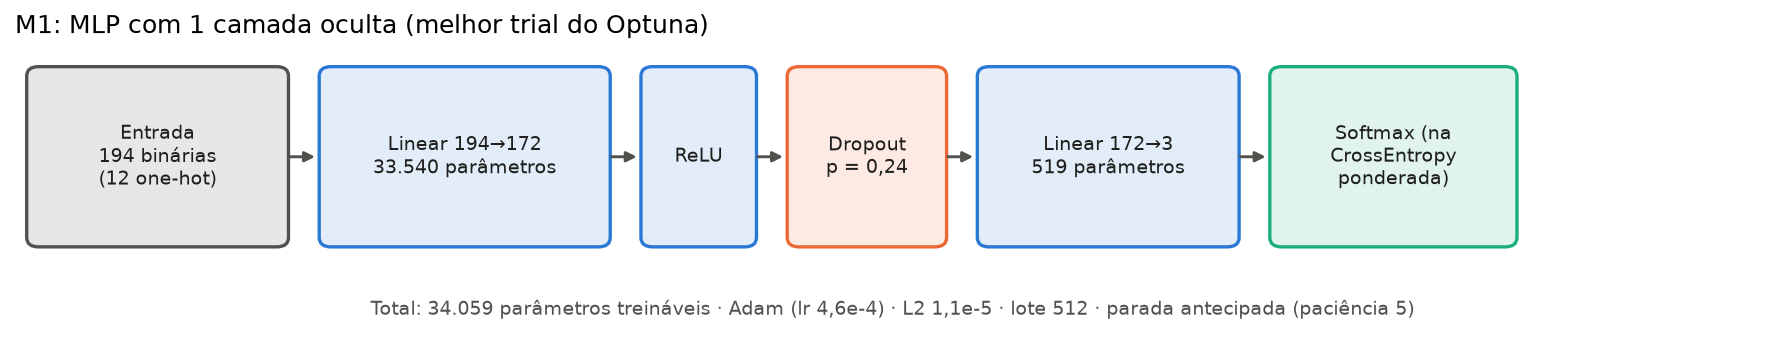
\includegraphics[width=0.62\textwidth]{figuras/16_arquitetura_m1}
  \caption{Arquitetura do modelo final (M1)}
  \label{fig:arq-m1}
  \fontefig{Elaborado pelo autor}
\end{figure}

Uma única função de treino, por épocas e \textit{mini-batches} com retropropagação do gradiente \cite{nielsen2015}, é usada na busca e nos modelos finais, com quatro regularizações: dropout após cada ReLU, L2 (\texttt{weight\_decay}), L1 (somada à perda como $\lambda \sum |w|$) e parada antecipada pelo Macro F1 de validação, que restaura os pesos da melhor época (paciência 4 na busca, 5 no treino final). A normalização por lote (BatchNorm) foi avaliada (Seção~\ref{sec:regularizacao}), mas não entrou nos modelos finais.

\section{Hiperparametrização: espaço de busca e configuração do estudo}
\label{sec:optuna}

A estratégia foi a busca bayesiana (\textit{Bayesian Search}), com o Optuna. Ao contrário do \textit{grid search}, que percorre toda a grade, e do \textit{random search}, que sorteia às cegas, ela usa os resultados anteriores para escolher a próxima tentativa: o amostrador TPE (\textit{Tree-structured Parzen Estimator}) concentra as tentativas nas regiões do espaço que vêm dando bons resultados. Isso importa aqui porque cada tentativa treina uma rede e o espaço tem sete hiperparâmetros.

Foram 25 tentativas, orçamento definido pelo tempo em CPU e suficiente porque as melhores convergem para a mesma região (Seção~\ref{sec:busca}), cada uma treinada numa subamostra estratificada de 300 mil linhas por até 15 épocas e avaliada na validação completa; o \texttt{MedianPruner} interrompe, a partir da 5\textsuperscript{a} época, as tentativas abaixo da mediana. A métrica otimizada foi o Macro F1 de validação, que dá o mesmo peso às três classes. O Quadro~\ref{qua:espaco} apresenta o espaço de busca e a justificativa de cada intervalo; otimizador, ativação e inicialização ficaram fora da busca por baixa influência esperada numa MLP rasa com entradas binárias.

\begin{quadro}[!htbp]
\caption{Espaço de busca e justificativa dos intervalos}
\label{qua:espaco}
\begin{center}
\footnotesize
\begin{tabularx}{\textwidth}{|P{2.6cm}|P{3.2cm}|Y|}
\hline
\textbf{Hiperparâmetro} & \textbf{Intervalo} & \textbf{Justificativa} \\ \hline
Taxa de aprendizado & $10^{-4}$ a $5 \cdot 10^{-3}$, escala log & em torno do padrão do Adam ($10^{-3}$), uma década abaixo e meia acima \\ \hline
Camadas ocultas & 1 a 3 & o teorema da aproximação universal \cite{hornik1989} garante uma camada em princípio, sem dizer quantos neurônios; mais camadas podem representar a mesma função com menos neurônios \cite{stathakis2009} \\ \hline
Neurônios por camada & 16 a 256, escala log, independente por camada & de uma compressão forte até cerca de 1,3 vez as 194 entradas; permite pirâmide ou mesma largura \\ \hline
Tamanho do lote & \{256, 512, 1024, 2048\} & lotes maiores aceleram cada época; menores introduzem ruído no gradiente que tende a generalizar melhor \\ \hline
Dropout & 0 a 0,5 & faixa usual de 10\% a 50\%, com a opção de desligar \\ \hline
L2 & $10^{-6}$ a $10^{-2}$, escala log & no M1 treinado $\sum w^2 \approx 447$; com $\lambda = 10^{-2}$ o termo já vale $\approx$2,2, três vezes a entropia cruzada \\ \hline
L1 & desligado ou $10^{-7}$ a $10^{-4}$, escala log & no M1 treinado $\sum |w| \approx 2.900$; com $\lambda = 10^{-3}$ o termo já valeria quatro vezes a entropia cruzada \\ \hline
\end{tabularx}
\end{center}
\fontequa{Elaborado pelo autor}
\end{quadro}

\section{Da hiperparametrização ao modelo final e protocolo de avaliação}
\label{sec:busca-final}

A Figura~\ref{fig:fluxo-final} resume o caminho até o modelo final. As 25 redes da busca só ranqueiam as combinações; as 3 melhores com arquiteturas distintas (M1, M2 e M3) são treinadas do zero com toda a base de treino (até 30 épocas, paciência 5) e avaliadas no teste. A subamostra de 300 mil linhas deixou a busca em 6 minutos, e o Macro F1 de validação passou de 0,600 na busca para 0,605 com a base inteira, o que indica que a região encontrada também é boa na base inteira.

A métrica principal é o Macro F1; as complementares são acurácia, precisão e \textit{recall} macro e matriz de confusão. O custo é medido por parâmetros, épocas e tempos de treino e inferência. Com as mesmas partições e o mesmo \textit{encoder}, foram feitos ainda um experimento controlado de largura $\times$ profundidade (um \textit{grid search} de 3 profundidades $\times$ 3 larguras, com o resto fixo) e a comparação técnica por técnica das regularizações, ambos na subamostra de 300 mil linhas da busca, e, com a base de treino completa, \textit{baselines} (incluindo regressão logística com o \texttt{C} escolhido numa grade de quatro valores) e a ablação por grupo de entradas. Todos os modelos usaram uma única semente.

\begin{figure}[!htbp]
  \centering
  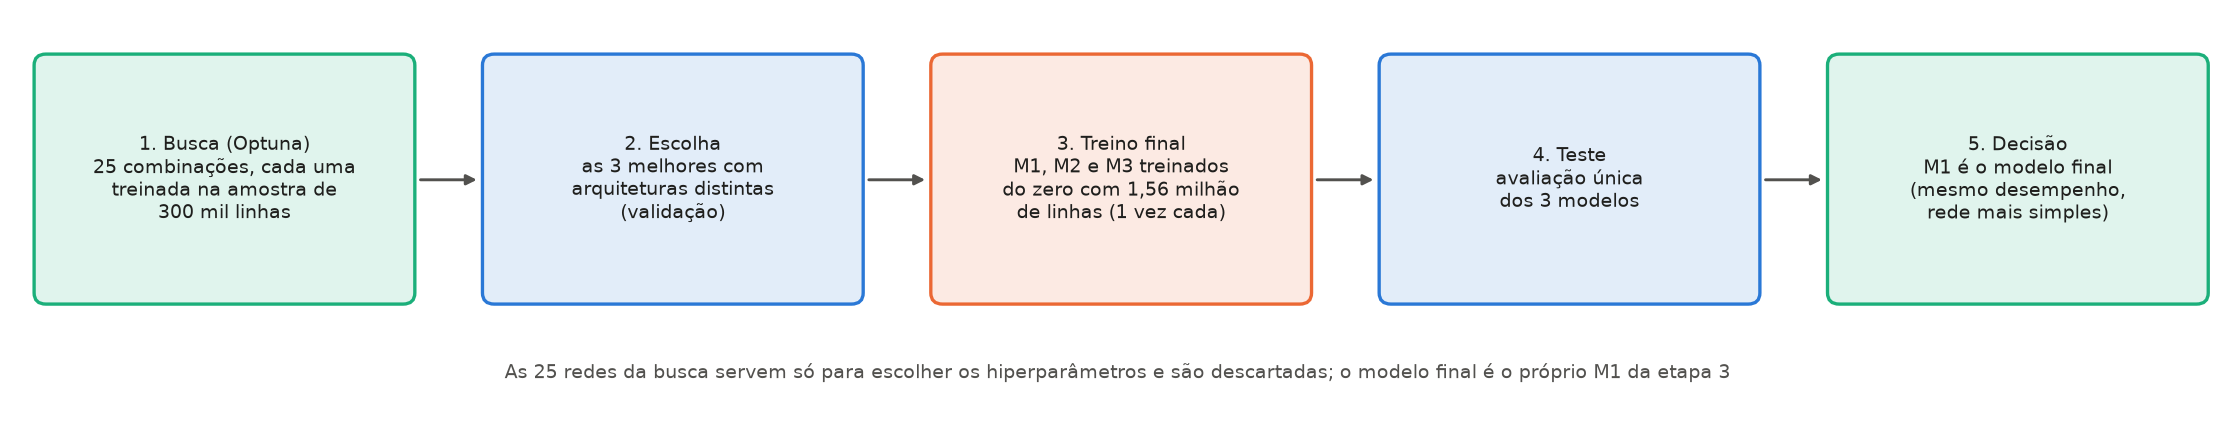
\includegraphics[width=0.7\textwidth]{figuras/19_fluxo_modelo_final}
  \caption{Da busca de hiperparâmetros ao modelo final}
  \label{fig:fluxo-final}
  \fontefig{Elaborado pelo autor}
\end{figure}
